\documentclass[14pt]{beamer}

\title[Infanzia]{The Infanzia Series}
\subtitle{Interactive Fun Learning Apps for kids}
\author[Team 16]{Rishika J, Sonal K, Akansha MP}
\date{August 31, 2020}

\usetheme{metropolis}
\usecolortheme{crane}
\usepackage{graphicx}
\usepackage{xcolor}


\begin{document}

\begin{frame}
    \titlepage
\end{frame}


\begin{frame}[standout]
    \alert{The Infanzia Series}
\end{frame}


\begin{frame}{Overview}
    \pause
    \begin{itemize}
    \item \textbf{Motive}: \\
            Interactive Enjoyable Applications
        \pause
    \item \textbf{Target Audience}: \\
            Pre-schoolers and Kindergartners
    \end{itemize}
\end{frame}


\begin{frame}[standout]
    \alert{The Series}
\end{frame}


\begin{frame}
    \begin{enumerate}
        \item \textbf{Word-it-Kid: English} \\
    \pause
        \item \textbf{Count-it-Kid: Maths} \\
    \pause
        \item \textbf{Know-it-Kid: EVS} 
    \end{enumerate}
\end{frame}


\begin{frame}{Techstack}
    \pause
    \begin{enumerate}
        \item Flutter
    \pause
        \item Dart
    \pause
        \item Firebase  
    \end{enumerate}
\end{frame}


\begin{frame}{Statistics}
    \pause
    \begin{itemize}
        \item 2 months
            \pause
        \item more than 3000 lines of code
            \pause
        \item 205 commits
    \end{itemize}
\end{frame}


\begin{frame}[standout]
    \alert{Features}
\end{frame}


\begin{frame}{Login}
    \pause
    Multi-User Login \\
    \pause
    Username and age as Input \\
    \pause
    Selection of Module: \\
    \begin{itemize}
    	\item Pre-school
        \item Kindergarten
    \end{itemize}
\end{frame}


\begin{frame}{Content}
    \begin{itemize}
            \pause
        \item Learn with fun exercises \\
            \pause
        \item Sing along rhymes \\
            \pause
        \item Play games \\
    \end{itemize}
\end{frame}


\begin{frame}[standout]
    \alert{Here's a quick demo \ldots}
\end{frame}


\begin{frame}[standout]
    \alert{Difficulties and Solutions}
\end{frame}


\begin{frame}{What and How?}
    \begin{enumerate}
        \item Integrating Images for login
            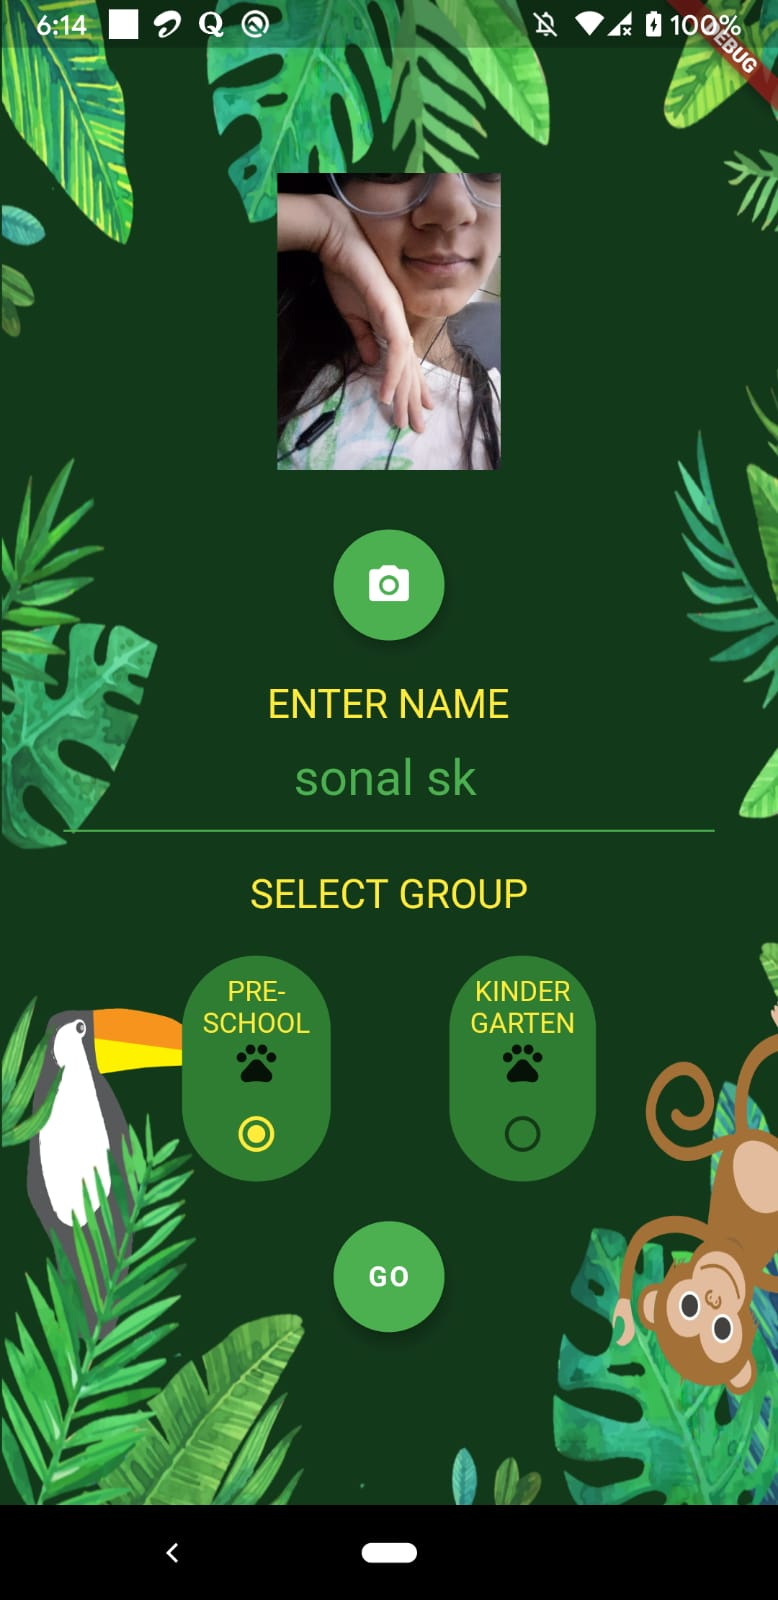
\includegraphics[width=0.9\textwidth]{Issue1}
            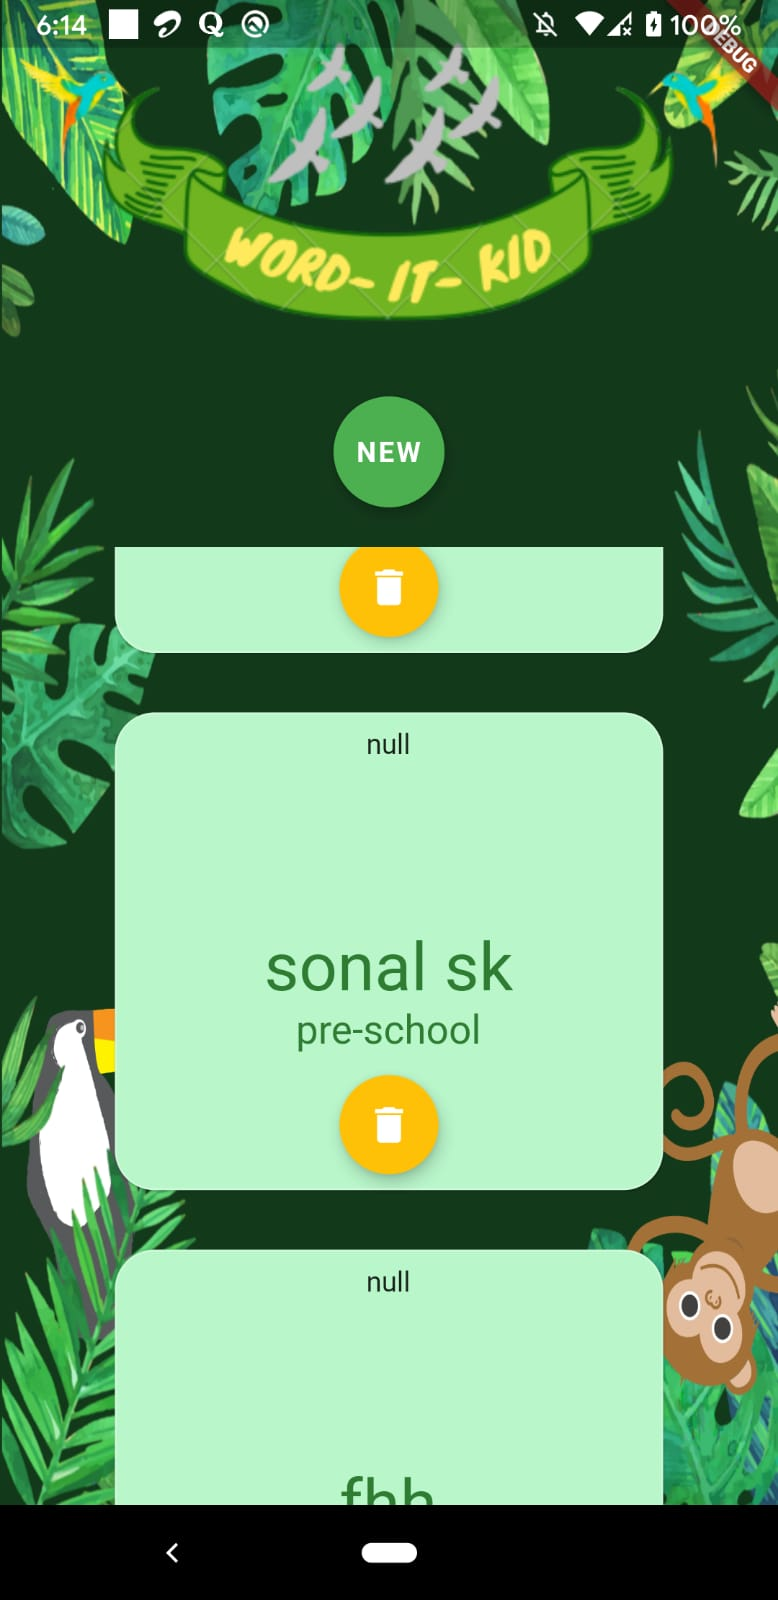
\includegraphics[width=0.9\textwidth]{Issue2}
            \includegraphics[width=0.9\textwidth]{Issue3}
    \end{enumerate}
\end{frame}


\begin{frame} {What and How?}
    \begin{enumerate}
        \item Integrating Images for Login
    \pause
        \item Adding Images in pubspec.yaml File
    \pause
        \item Text to Speech
    \pause
        \item Clickable Flash Cards
    \pause
        \item Scrollview to Sliderview
    \pause
        \item Random Generator
    \pause
        \item Push-Pop Navigation
    \pause
        \item Integrating Audio with Flip Cards
    \end{enumerate}
\end{frame}


\begin{frame}[standout]
    \alert{Learnings}
\end{frame}

\begin{frame}{Learnings}
    \begin{enumerate}
    \pause
        \item Making Applications with Flutter 
    \pause
        \item Integrating Firebase
    \pause
        \item Splashscreen
    \pause
        \item Integrating Whiteboard
    \pause
        \item Advanced UI Features
    \end{enumerate}
\end{frame}


\begin{frame}[standout]
   Future Scope 
\end{frame}


\begin{frame}{References}
    \begin{enumerate}
        \item Flutter Documentation
        \item YouTube
        \item pub.dev
    \end{enumerate}
\end{frame}


\begin{frame}[standout]
    \alert{Any Questions?}
\end{frame}


\end{document}
